\documentclass{article}
\usepackage{amsmath}
\usepackage{geometry}
%\usepackage[]{mcode}
\usepackage{graphicx}
\usepackage{float}
\usepackage{placeins}
\usepackage{gensymb}

\geometry{
left = 1.25in,
lmargin = 1.25in,
inner = 1.25in,
right = 1.25in,
rmargin = 1.25in,
outer = 1.25in,
top = 1in,
tmargin = 1in,
bottom = 1in,
bmargin = 1in,
}

\begin{document}

\title{Inverted Pendulum Controllers}
\author{Garrett Wilson and Nathan Zimmerly \\ \\
ENGR 352}
\maketitle

\clearpage

\tableofcontents

\pagebreak

\section{PID Controller}
Can add if you want Garrett. I have it all written up in a seperate document.

\section{LQR State Space Controller}
\subsection{4th Order}
\subsubsection{State-Space Modeling}
Below is the free-body diagram of the inverted pendulum and cart

\begin{figure}[!htb]
\centering
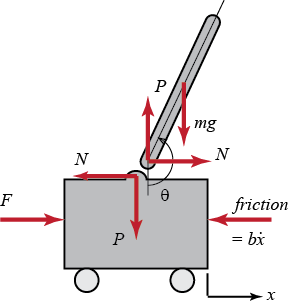
\includegraphics{pendulumfbd}
\caption{Source: http://ctms.engin.umich.edu/}
\end{figure}

Summation of carts forces in the horizontal direction
\begin{equation} 
\label{eqn1}
F = M\ddot{x}+b\dot{x} + N
\end{equation}

Summation of the pendulum forces in the horizontal direction
\begin{equation} 
\label{eqn2}
N = m\ddot{x}+m l \ddot{\phi} cos(\phi)-m l \dot{\phi}^2sin(\phi)
\end{equation}

Substituting \ref{eqn2} into \ref{eqn1}
\begin{equation} 
\label{eqn3}
F = M\ddot{x}+b\dot{x} + m\ddot{x}+m l \ddot{\phi} cos(\phi)-m l \dot{\phi}^2sin(\phi)
\end{equation}

Next, the sum of forces perpendicular to the pendulum
\begin{equation} 
\label{eqn4}
Psin(\phi)+Ncos(\phi)-mgsin(\phi) = m l \ddot{\phi} + m\ddot(x)cos(\phi)
\end{equation}

Summing tthe moments about the centroid of the pendulum
\begin{equation} 
\label{eqn5}
-P sin(\phi)-N cos(\phi) = I \ddot{\phi}/l
\end{equation}

Combining \ref{eqn4} and \ref{eqn5} leads to 
\begin{equation} 
\label{eqn6}
(I+m l^2)\ddot{\phi} + m g lsin(\phi) = -m l \ddot{x} cos(\phi)
\end{equation}

Small angle approximations. $\theta$ \textrm{ replaces } $\phi$ \textrm{ so that the angle } $\theta$ \textrm{ = 0} $\degree$ \textrm{ is straight up}.
\\

\begin{equation} 
\label{sa1}
cos(\phi) = cos(\pi + \theta) \approx -1
\end{equation}

\begin{equation} 
\label{sa2}
sin(\phi) = sin(\pi + \theta) \approx -\theta
\end{equation}

\begin{equation} 
\label{sa3}
\dot{\phi} = \dot{\theta} \approx 0
\end{equation}

Plugging \ref{sa1} and \ref{sa2} into \ref{eqn3} and \ref{eqn6} leads to
\begin{equation} 
\label{eqn3b}
F = (M+m)\ddot{x}+b\dot{x} -m l \ddot{\theta}
\end{equation}

\begin{equation} 
\label{eqn6b}
(I+m l^2)\ddot{\theta} - m g l\theta = m l \ddot{x}
\end{equation}

Motor Equations
\begin{equation} 
\label{eqn7}
L i + R i = V - k_m\dot{\theta}
\end{equation}

\begin{equation} 
\label{eqn8}
\tau = k_m*i
\end{equation}
To arrive at state space equations add \ref{eqn7} and \ref{eqn8} into \ref{eqn3b} and \ref{eqn6b}. Note: L = 0.

Plugging \ref{eqn8} into \ref{eqn7} leads to 
\begin{equation} 
\label{eqn9}
F = \frac{R k_m}{r(V-k_m\dot{\theta})}
\end{equation}

Finally, plugging \ref{eqn9} into \ref{eqn3b} and \ref{eqn6b} and solving for $\ddot{x}$ and $\ddot{\theta}$ leads to the state space equations below

\begin{equation}
\label{ss1}
\begin{bmatrix}
\dot{x}\\
\ddot{x}\\
\dot{\theta}\\
\ddot{\theta}\\
\end{bmatrix} =
\begin{bmatrix}
0&1&0&0\\
0&\frac{(I+m l^2)/(m l) (-(b+K^2/(R r^2))}{(M+m) (I+m l^2)/(m l)-m l}&\frac{(I+m l^2)/(m l) (M+m) g}{[(M+m) 		(I+m l^2)/(m l)-m l]-g}&0\\
0&0&0&1\\
0&\frac{-(b+K^2/(R r^2))}{(M+m) (I+m l^2)/(m l)-m l}&\frac{(M+m) g}{(M+m) (I+m l^2)/(m l)-m l}&0\\
\end{bmatrix}
\begin{bmatrix}
x\\
\dot{x}\\
\theta\\
\dot{\theta}\\
\end{bmatrix} +
 	\begin{bmatrix}
0\\
\frac{(I+m*l^2)/(m*l)*(K/(R*r)}{(M+m) (I+m l^2)/(m l)-m l}\\
0\\
\frac{K/(R*r)}{(M+m) (I+m l^2)/(m l)-m l}\\
\end{bmatrix} v
\end{equation}
  
\begin{equation}
\label{ss2}
\begin{bmatrix}
x\\
\theta \\
\end{bmatrix} =
\begin{bmatrix}
1&0&0&0\\
0&0&1&0\\
\end{bmatrix}
\begin{bmatrix}
x\\
\dot{x}\\
\theta\\
\dot{\theta}\\
\end{bmatrix}
\end{equation}

\subsubsection{Poles, Stability, and Observability}
Now that the state-space equations are found, the poles of the model are equal to the eigen values of the A matrix. The original Poles are shown below:
\begin{enumerate}
  \item   0.00000 + 0.00000i
  \item -9.9916 + 0.00000i
  \item -4.9981 + 0.00000i
  \item 5.1345 + 0.00000i
\end{enumerate}
Because one of the poles is positive, the system is unstable. We will fix this with a controlled matrix A in the next section.

If the rank of the controllability matrix shown below equals the number of states the system (n) is made up of, then the system is controllable. In our case the rank of R equals 4 so our system is controllable. This means that our system can reach any state.

\begin{equation} 
\label{ctrb}
\centering
R = \begin{bmatrix}
	B&AB&\hdots&A^{n-1}B\\
	\end{bmatrix}
\end{equation}
 
 If the rank of the observability matrix shown below equals the number of states the system is made up of, then the system is observable. In our case the rank of O eqauls 4 so our system is observable. This means that in any possible situation, the current state of our system can be determined using only the outputs.
 
 \begin{equation} 
\label{obsv}
\centering
O = \begin{bmatrix}
	C\\
	CA\\
	\vdots\\
	CA^{n-1}\\
	\end{bmatrix}
\end{equation}

\subsubsection{LQR Controller}
A linear-quadratic regulator (LQR) weights factors depending on their importance using the nxn Q matrix, while minimizing another factor using the variable R. In our case, the weighted factors were the position of the cart (x) and the angle of the pendulum ($\theta$). Also, the factor that we minimized is the velocity of the cart. A good starting point for Q is C'C evenly weighting the factors. However, we care much more about the pendulum staying vertical than we do the position staying at 0 m. Because of this, after some tests we weighted x at 1000 and $\theta$ at 100,000. leaving the Q matrix below. Also, a good place to start the limiting factor is 1, but we change R = 0.1.

 \begin{equation} 
\label{q}
\centering
Q = \begin{bmatrix}
	1000&0&0&0\\
	0&0&0&0\\
	0&0&100,000&0\\
	0&0&0&0\\
	\end{bmatrix}
\end{equation}

In LQR controllers, the state-feedback control gains vector k is used to move the poles in the system. It can be calculated by minimizing the cost function J. We used Octave's LQR function to calculate our k vector. Once calculated, the corrected A matrix can be calculated using the equation below.

\begin{equation}
\label{ac}
A_c=[A-Bk]
\end{equation}

\subsubsection{Precompensator}
At this point, our pendulum seemed to stay up, but the cart would not stay at the center. Because of this, we had to add a precompensator to account for steady-state error. Because the cart's position had steady-state error, we chose the C matrix below.
\\

\begin{equation}
\label{pcomp}
\centering
C_n = [1 0 0 0]
\end{equation}
 
 By replacing the state space C matrix with C\_n, $\bar{N}$ can be calculated. We used Octave's rscale function to calulate $\bar{N}$. $\bar{N}$ is a scale factor that eliminates the stead-state error of a system to a step input. It should be noted that $\bar{N}$ only works for single input systems, which is why we could use it to only eliminate the steady state error in the carts position. Once $\bar{N}$ is calculated, the state space equation uses the corrected A matrix, B $\bar{N}$, C, and D for the A, B, C, and D matrices respectively.
 
 \subsubsection{Adding an Observer-Based Estimator}
 Previous work assumes full-state feedback, which means that x, $\dot{x}$, $\theta$, and $\dot{\theta}$ are all being measure. However, only x and $\theta$ are being measured so we must add observer based control. Below are the previous block diagram, and the updated block diagram with the observer-based estimator.

\begin{figure}[!htb]
\centering
  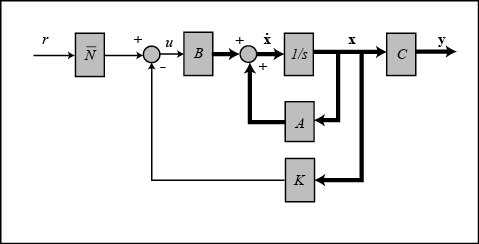
\includegraphics[width=.7\linewidth]{blockd}
  \caption{Original}
  \label{bd}
  \end{figure}

\begin{figure}[!htb]
  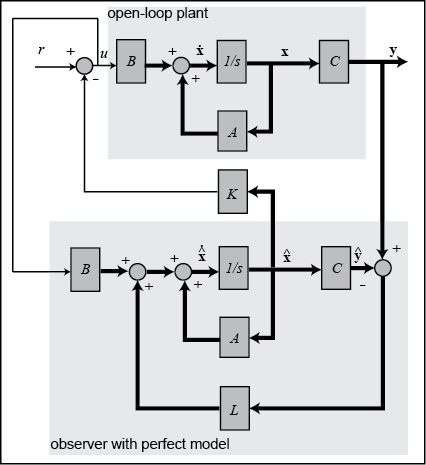
\includegraphics[width=.6\linewidth]{observer_blockd}
  \caption{With Precompensator}
  \label{bd2}
\end{figure}


\clearpage

The speed of convergence depends on the poles of the estimator. Since we are going to use the estimation before the actual event accurs, we want the estimation to converge must faster. Because of this we want the poles of our estimator to be at least four times faster than the slowest controller pole. If the estimator poles are too fast it can cause error in the measurement, so usually the poles of the estimator should not be more than 10 times larger than the smallest controller pole. Also, the estimator poles should be close together. The current poles of our C matrix are listed below. Placing the estimator poles P at [-30, -31, -32, -33] was found to work after several trials. Note: we did not place all the estimator poles in the same position because the Octave place function used to find L does not support that.
\begin{enumerate}
  \item  -50.8860 +50.1382i
  \item -50.8860 -50.1382i
  \item -0.7136 + 0.6863i
  \item -0.7136 - 0.6863i
\end{enumerate}

Based on the estimator poles, we placed the Octave place function which computes L. Based on the Original A, B, C, and D matrices for state space, the final state space equations are shown below:

\begin{equation}
\label{ss3}
\begin{bmatrix}
\dot{x}\\
\dot{e}\\
\end{bmatrix}
=
\begin{bmatrix}
A-Bk&Bk\\
0&A-LC\\
\end{bmatrix}
\begin{bmatrix}
x\\
e\\
\end{bmatrix} +
\begin{bmatrix}
B\bar{N}\\
0\\
\end{bmatrix} r
\end{equation}

\begin{equation}
\label{ss4}
y = 
\begin{bmatrix}
C&0\\
\end{bmatrix}
\begin{bmatrix}
X\\
e\\
\end{bmatrix} +
\begin{bmatrix}
0\\
\end{bmatrix} r
\end{equation}

\subsection{6th Order}
%Should we just talk about what we had or show derivations?

\section{Future Work}
Future work for this pendulum includes using a UFIR or kalman filter to eliminate error from noise. Currently, the Pendulum works (with the wrong radius value), but it does have some noise cause it to rock back and forth. A kalman filter should help quite efficiently, however error matrices have to be found through tests which is difficult. There is another way to calculate the error matrices through iteration and there is an octave package called ALS which is supposed to help find them. The UFIR method is more complex, making more work for the computer running the program. However, it works significantly than the original kalman filter, unless the error matrices are exact in which case the kalman filter is slightly better. We have spent time trying to get both methods to work without success, however we're fairly certain that if we had more time we could get at least one of the methods to work.


\end{document}